\documentclass[12pt,a4paper]{report}
\usepackage{amsmath, amssymb, amsfonts}
\usepackage{graphicx}
\usepackage{subcaption}  
\usepackage{caption}
\usepackage{geometry}
\usepackage{enumitem}
\usepackage{listings}
\usepackage{xcolor}
\usepackage{hyperref}
\usepackage{cleveref}
\hypersetup{
    colorlinks=true,
    linkcolor=blue,
    citecolor=blue,
    urlcolor=blue,
    pdfauthor={Akhil CV},
    pdftitle={Limit Order Book - Market Making}
}
\usepackage{booktabs}
\usepackage{array}
\usepackage{multirow}
\usepackage{siunitx}
\usepackage{multicol}
\usepackage{algorithm}
\usepackage{algorithmic}
\usepackage[backend=biber,style=authoryear]{biblatex}

\addbibresource{ref.bib}

\geometry{margin=1in}

\begin{document}

% ================= TITLE PAGE =================
\begin{titlepage}
\begin{center}
{\Large Master Thesis Project Report}\\[1.2cm]
\large{on}\\[1.2cm]
\linespread{1.2}\LARGE {\bfseries MTP 2: Limit Order Book - Framework for Market Making}\\[1.2cm]

\large{by}\\[1.2cm]
{\large\textbf{Akhil CV}}\\
\large{(Roll No. 24M1530)}\\[1.2cm]

\large{\textbf{Supervisor:}}\\
\large{\textbf{Prof. K.S. Mallikarjuna Rao}}\\[1cm]

\linespread{1}


\includegraphics[width=6cm]{IIT_logo.jpg}\\[0.5cm]

\large Department of Industrial Engineering and Operations Research  \\[0.3cm] 
\large Indian Institute of Technology, Bombay\\
\large Mumbai 400076 (India)
\end{center}
\end{titlepage}

% ================= PAGE NUMBERING =================
\pagenumbering{roman}

% Optional: Abstract / Preface can go here

\newpage
\pagenumbering{arabic}

\newpage
\begin{center}
    {\LARGE \textbf{Declaration}}
\end{center}

\vspace{1em}

\noindent
I declare that this written submission represents my ideas in my own words and where others’ ideas or words have been included, I have adequately cited and referenced the original sources. I declare that I have properly and accurately acknowledged all sources used in the production of this report. I also declare that I have adhered to all principles of academic honesty and integrity and have not misrepresented or fabricated or falsified any idea/data/fact/source in my submission. I understand that any violation of the above will be a cause for disciplinary action by the Institute and can also evoke penal action from the sources which have thus not been properly cited or from whom proper permission has not been taken when needed.

\vspace{2cm}

\noindent
\begin{minipage}[t]{0.5\textwidth}
    \textbf{Date:} xx May 2026
\end{minipage}%
\begin{minipage}[t]{0.5\textwidth}
    \raggedleft
    \rule{5cm}{0.4pt}\\
    Akhil CV\\
    (Roll No. 24M1530)
\end{minipage}

%\end{Declaration}

\section*{\centering Acknowledgement}
\vspace{4mm}
I would like to extend my deepest gratitude to my supervisors, Prof. K.S. Mallikarjuna Rao and Prof. Veeraruna Kavitha, whose guidance, encouragement, and constructive feedback have been instrumental in shaping this work. Their patience and expertise have consistently motivated me to push the boundaries of my understanding and strive for excellence.\vspace{3mm}

\noindent I am thankful to the Department of Industrial Engineering and Operations Research (IEOR), IIT Bombay, for providing a vibrant academic environment and access to the resources that made this research possible.\vspace{3mm}

\noindent I am forever grateful to my parents and friends for their unwavering love, encouragement, and belief in me. Their support has been a constant source of strength and inspiration throughout this journey.\vspace{3mm}

\noindent I am truly indebted to all those who have contributed to the realization of this thesis, and I express my sincerest thanks to each and every one of them.


\section*{\centering Abstract}
\vspace{4mm}
dvam.kfmcams.,mc


\clearpage

% ================= MAIN TITLE =================
\title{MTP 2: Limit Order Book - Framework for Market Making}
\author{Prepared by: Akhil CV (24M1530) \\ Guided by: Prof. K.S. Mallikarjuna Rao}
\date{}

\maketitle


\newpage
\tableofcontents
\clearpage
\listoffigures
\clearpage
% \listoftables
\clearpage

\cleardoublepage
\pagenumbering{arabic}
\setcounter{page}{1}
% ================= CONTENT START =================
\chapter{Introduction} 
\thispagestyle{plain}
% \section{Introduction}

Modern financial markets are predominantly organized around the \textit{limit order book} (LOB), a set of digital instruction  through which market participants submit buy and sell orders at specified prices and quantities. The LOB provides a detailed and dynamic representation of market microstructure, capturing the continuous interaction between supply and demand. With the widespread availability of high-frequency data, advances in computational power, and the rapid growth of algorithmic and data-driven trading strategies, the analysis of LOB data has become central to quantitative finance.

At a granular level, the LOB reflects the process of price formation, where the evolution of bid and ask queues determines the execution of trades and the emergence of price dynamics. In addition to providing insights into liquidity and order flow, historical LOB data enables practitioners to reconstruct past market conditions, simulate trading environments, and evaluate execution strategies. As a result, modeling and understanding LOB dynamics is of significant importance for applications such as market making, optimal execution, and high-frequency trading.

A large body of literature has focused on modeling the LOB from both theoretical and empirical perspectives. The work of \cite{ref2} develops a Markovian framework for the LOB, providing a rigorous treatment of its stochastic properties, including recurrence behavior and implications for trading strategies. More broadly, recent surveys and empirical studies highlight a range of approaches for LOB modeling, including queueing models, stochastic processes, agent-based simulations, and machine learning techniques. These models aim to capture key stylized facts such as heavy-tailed distributions, long memory, and state-dependent dynamics.

\cite{ref1}
\cite{ref3}
\cite{ref4}

Despite these advances, several challenges remain. First, many classical approaches rely on strong  assumptions and often fail to capture the complex, nonlinear, and non-stationary nature of modern financial markets. Second, purely data-driven methods such as clustering algorithms may overlook the temporal dependencies inherent in LOB dynamics, leading to suboptimal representations of market regimes. Third, while significant effort has been devoted to predicting price movements, comparatively less attention has been given to integrating regime identification with execution-aware strategies, particularly in the context of market making.

\section{Literature Gap}

Existing approaches to LOB modeling can broadly be categorized into parametric models, statistical learning methods, and deep learning-based approaches. Parametric models, such as Markovian or stochastic process-based frameworks, provide interpretability but often lack flexibility in capturing real-world complexities. On the other hand, machine learning methods, including clustering and neural networks, offer greater expressive power but may ignore temporal structure or lack interpretability.

A key limitation across these approaches is the disconnect between \textit{regime identification} and \textit{execution strategy design}. While regime-switching models and clustering techniques can identify different market states, they are rarely integrated into a unified framework that directly informs trading decisions. In particular, most existing works do not explicitly model the relationship between order placement, execution probability, and profitability within different market regimes.

Furthermore, standard clustering methods such as K-means treat observations as independent, neglecting the sequential and path-dependent nature of LOB data. This limits their effectiveness in capturing regime persistence and transitions, which are critical for high-frequency trading strategies. There is therefore a need for a framework that combines regime detection with execution modeling, while remaining computationally tractable and adaptable to real-time applications.

\section{Contributions}

In this paper, we propose a unified framework for modeling the limit order book with a focus on market making strategies. The main contributions are as follows:

\begin{enumerate}
    \item \textbf{Regime Identification:} We introduce a data-driven approach to partition LOB states into distinct regimes using clustering techniques. While we begin with K-means as a baseline due to its simplicity and scalability, the framework is designed to accommodate more advanced models that incorporate temporal dependencies and stochastic dynamics.

    \item \textbf{Online Regime Classification:} We develop a mechanism to classify incoming market data into the identified regimes in real time. This enables adaptive decision-making by continuously updating the market state based on observed order flow and liquidity conditions. This also opens up the opportunity to pursue research in the direction of reinforcement learning.

    \item \textbf{Execution Probability Modeling:} We propose a methodology to estimate execution probabilities for limit orders as a function of their distance from the midprice. This allows us to quantify the trade-off between execution likelihood and spread capture, which is central to market making strategies.

    \item \textbf{Market Making Framework:} By integrating regime identification and execution modeling, we construct a systematic approach for placing bid and ask orders. The framework aims to exploit favorable market conditions, maximize spread capture, and improve profitability while managing inventory risk.

    \item \textbf{Scalable Pipeline:} The proposed approach is designed to be computationally efficient and scalable, making it suitable for high-frequency environments where real-time processing of LOB data is essential.
\end{enumerate}

\section{Paper Organization}

The remainder of the paper is structured as follows. Section 2 describes the representation of the limit order book, construction of microstructure features. This section states some possible features that are relevant in making decisions pertaining to market making. It also provide the future scope of research and implementation on this segment.  Section 3 presents the regime identification methodology. Section 4 develops the execution probability model and market making strategy. Section 5 discusses the implemented pipeline and outlines directions for future research.

\chapter{Representation of the Limit Order Book}

The limit order book (LOB) provides a granular view of market liquidity by recording outstanding buy and sell orders at discrete price levels. At any given time, the LOB consists of two sides: the bid side (buy orders) and the ask side (sell orders), each organized by price and associated volume. In this work, we utilize level-2 data with a fixed depth of 20 levels on each side of the book.

Let the market data consist of a sequence of order book events

\[
\mathcal{D} = \{(t_i, s_i, p_i, q_i)\}_{i=1}^{N}
\]

where

\begin{itemize}
\item $t_i$ denotes the timestamp,
\item $s_i \in \{\text{Bid}, \text{Ask}\}$ denotes the order side,
\item $p_i$ denotes the order price,
\item $q_i$ denotes the order quantity.
\end{itemize}

Each order book state is grouped by a snapshot index rather than any time unit. This will vary significantly according to the availability of the technology. For instance, on 11 Apr 2026, NSE has cut its response time to nano second from existing millisecond. The implication is  availability of data and trades at ultra low latency. We thus define our discretization by the smallest observable data feed.

\[
\text{snap\_idx} = k
\]

representing the set of orders active at that instant.

In order to characterize the state of the limit order book (LOB), several microstructure features are constructed from the bid and ask prices and volumes. Let

\begin{itemize}
\item $P_i^b(t)$ denote the bid price at level $i$ at time $t$
\item $P_i^a(t)$ denote the ask price at level $i$ at time $t$
\item $V_i^b(t)$ denote the bid volume at level $i$ at time $t$
\item $V_i^a(t)$ denote the ask volume at level $i$ at time $t$
\end{itemize}

where $i = 1,2,\dots,L$ and $L$ represents the number of depth levels observed in the order book (typically $L=20$). Level $i=1$ corresponds to the best bid and best ask.

\section{Best Bid and Best Ask}

For each snapshot $k$, the best bid and ask prices are defined as

\[
B_k = \max_{i:s_i=\text{Bid}} p_i
\]

\[
A_k = \min_{i:s_i=\text{Ask}} p_i.
\]

The corresponding queue sizes are denoted

\[
Q_k^{bid}, \qquad Q_k^{ask}.
\]

The Level--1 order book state is therefore

\[
X_k = (B_k, A_k, Q_k^{bid}, Q_k^{ask}).
\]

\section{Midprice and Price Normalization}

The midprice represents the midpoint between the best bid and ask:

\[
M_k = \frac{B_k + A_k}{2}.
\]

To analyze the relative structure of the book around the midprice, prices are normalized as

\[
p_i^{norm} = p_i - M_k.
\]

This representation centers the order book around zero, allowing symmetric analysis of bid and ask liquidity.


\section{Mid-Price Definition}

A fundamental reference point in LOB analysis is the \textit{mid-price}, defined as the average of the best bid and best ask prices:
\begin{equation}
    m_t = \frac{p_t^{\text{bid},1} + p_t^{\text{ask},1}}{2},
\end{equation}
where $p_t^{\text{bid},1}$ and $p_t^{\text{ask},1}$ denote the best (top-of-book) bid and ask prices at time $t$, respectively. The mid-price serves as a proxy for the fair value of the asset and is commonly used as a reference for price normalization and short-term price dynamics.
Under this representation, the mid-price is mapped to zero, bid prices take negative values, and ask prices take positive values. This normalization centers the LOB and allows for a symmetric visualization of liquidity around the prevailing market price.

\section{LOB Snapshot Representation}

A snapshot of the LOB is represented as a set of price-volume pairs for both bid and ask sides:
\[
\{(p^{\text{bid}}_i, v^{\text{bid}}_i)\}_{i=1}^{L}, \quad
\{(p^{\text{ask}}_i, v^{\text{ask}}_i)\}_{i=1}^{L},
\]
where $L=20$ denotes the depth of the book, $p_i$ represents the price level, and $v_i$ denotes the corresponding available volume.

For visualization, the LOB is often depicted as a bar plot in which:
\begin{itemize}
    \item The horizontal axis corresponds to price levels,
    \item The vertical axis represents available volume,
    \item The height of each bar reflects the liquidity available at that price level.
\end{itemize}
Bid volumes are typically shown on the left side and ask volumes on the right side, highlighting the asymmetry in liquidity across the book.

\begin{figure}[ht]
    \centering
    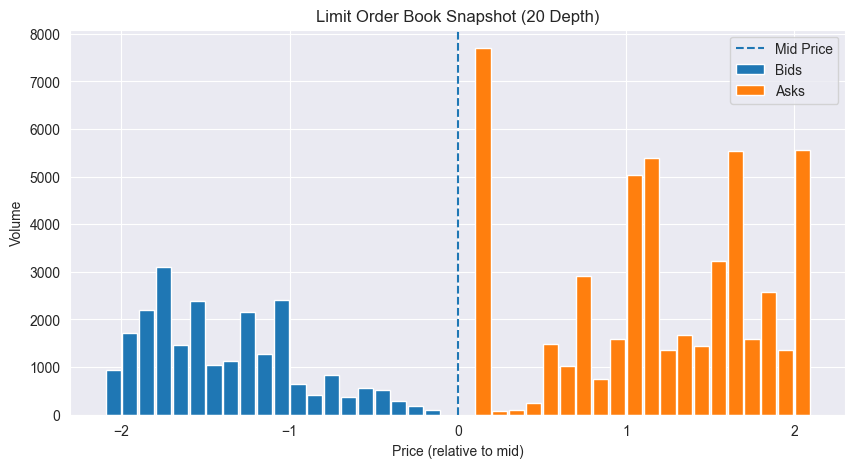
\includegraphics[width=0.9\linewidth]{LOB_snapshot.png}
    \caption{Snap shot of Limit order book}
    \label{fig:Snap shot of Limit order book}
\end{figure}

\section{Order Flow Imbalance}

In addition to static snapshots, the dynamics of the LOB can be summarized using the \textit{order flow imbalance} (OFI), which captures the relative dominance of buying versus selling pressure. A simple volume-based definition is given by:
\begin{equation}
    \text{OFI}_t = \frac{\sum_{i=1}^{L} v^{\text{bid}}_i - \sum_{i=1}^{L} v^{\text{ask}}_i}{\sum_{i=1}^{L} v^{\text{bid}}_i + \sum_{i=1}^{L} v^{\text{ask}}_i}.
\end{equation}
This measure takes values in $[-1,1]$, where positive values indicate bid-side dominance (buying pressure), and negative values indicate ask-side dominance (selling pressure).

\begin{figure}[ht]
    \centering
    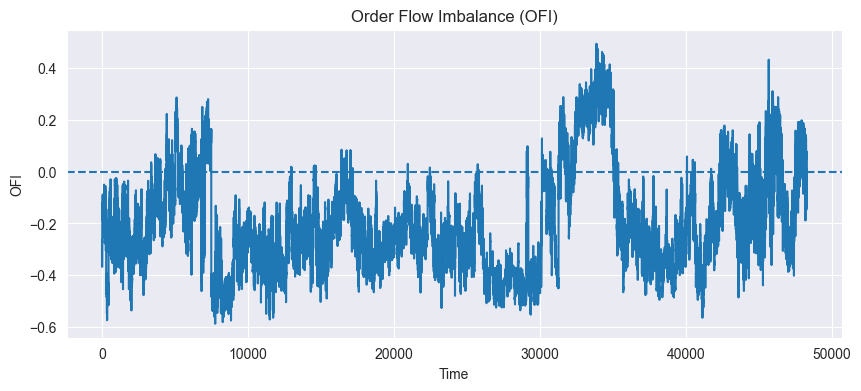
\includegraphics[width=0.9\linewidth]{orderflow_imbalance.png}
    \caption{orderflow}
    \label{fig:Representation of order flow imbalance}
\end{figure}

\section{Interpretation}

The combined representation of LOB snapshots and order flow imbalance provides both a static and dynamic view of market liquidity. While the snapshot reveals the distribution of available liquidity across price levels, the imbalance metric summarizes directional pressure in the market. Together, these representations are essential to understand short-term price formation, liquidity provision, and execution dynamics. 
As evident from the representation, it is clear that the depth under consideration can significantly alter this feature. The vast size of data and its storage and also computation required to effectively model at microstructural level, the selection of depth towards assessing orderflow imbalance is a research topic in itself.
 

\section{Microprice}

The microprice is a liquidity-weighted estimate of the efficient price:

\[
m_t =
\frac{A_t Q_t^{bid} + B_t Q_t^{ask}}
     {Q_t^{bid} + Q_t^{ask}}.
\]

This quantity tilts toward the side with greater available liquidity. Most of the charts and commercial data provides mid-price as the feature representing historical time series. It is however, prudent to note that the mid-price equally weight the bid and ask volumes. It is also known that the price dynamic is also dependent on the supply and demand for an instrument. Thus the suitability of microprice over midprice as a feature to represent evolution of prices is an interesting problem.

\section{Microprice Return}

We define the microprice return as

\[
r_t =
\log\left(\frac{m_t}{m_{t-1}}\right).
\]

\section{Order Book Imbalance}

The order book imbalance measures the relative strength of bid and ask liquidity:

\[
I_t =
\frac{Q_t^{bid} - Q_t^{ask}}
     {Q_t^{bid} + Q_t^{ask}}.
\]

Similar to flow imbalance, order book imbalance can depicts the pure tilt. 

\section{Volume Pressure}

A logarithmic liquidity ratio is defined as

\[
V_t =
\log\left(
\frac{Q_t^{bid}+1}{Q_t^{ask}+1}
\right).
\]

The feature vector used for regime detection is therefore

\[
Y_t = (r_t, S_t, I_t, V_t).
\]

\section{Queue Imbalance}

Queue imbalance focuses on the best bid and best ask queues. It measures the relative size of the order queues at the top of the book and is defined as

\[
QI_t =
\frac{V_1^b(t) - V_1^a(t)}
{V_1^b(t) + V_1^a(t)}
\]

Large positive values indicate stronger bid-side queue dominance.

\section{Depth Slope}

Depth slope measures how liquidity is distributed across different levels of the order book. One common formulation is

\[
Slope =
\frac{\sum_{i=1}^{L} i \cdot V_i}
{\sum_{i=1}^{L} V_i}
\]

A higher slope indicates that liquidity is concentrated further away from the best price levels.

\section{Order Flow Difference}

Order flow imbalance captures changes in the best bid and ask queue volumes over time. It is defined as

\[
OFI_t =
\left(V_1^b(t) - V_1^b(t-1)\right) -
\left(V_1^a(t) - V_1^a(t-1)\right)
\]

Positive values indicate net buying pressure in the order book.

\subsection{Cancellation Rate}

Cancellation rate measures how quickly resting orders are removed from the order book. If $C_t$ denotes the total cancelled volume during a time interval $\Delta t$, then the cancellation rate is

\[
CancellationRate_t =
\frac{C_t}{\Delta t}
\]

In practice, cancellations can be approximated by decreases in order book volume not associated with trades.

\section{Order Arrival Rate}

Order arrival rate measures the intensity of new limit orders entering the order book. If $A_t$ denotes the total volume of newly submitted orders within a time interval $\Delta t$, then

\[
ArrivalRate_t =
\frac{A_t}{\Delta t}
\]

This feature captures the rate at which liquidity is replenished in the market.

\chapter{Regime Selection}

\section{Motivation}

Financial markets exhibit distinct structural phases, commonly referred to as \textit{regimes}, which differ in terms of liquidity, volatility, and order flow dynamics. Identifying such regimes is crucial for market making, as the profitability of providing liquidity is highly dependent on prevailing market conditions. In particular, periods of stable price dynamics and balanced order flow are more suitable for market making, whereas strongly directional or highly volatile regimes can lead to adverse selection and increased execution risk.

This chapter focuses on the identification of such regimes using limit order book (LOB) data and the subsequent integration of regime information into a market making framework.

\section{Feature Construction from Limit Order Book}

To characterize market conditions, we extract a set of microstructure features from LOB snapshots. For each snapshot, we compute:

\begin{itemize}
    \item \textbf{Spread:} Difference between best ask and best bid prices.
    \item \textbf{Order Imbalance:} A measure of relative dominance of bid and ask volumes.
    \item \textbf{Bid Depth:} Aggregate volume on the bid side.
    \item \textbf{Ask Depth:} Aggregate volume on the ask side.
\end{itemize}

Formally, for each time step $t$, we construct a feature vector:
\[
X_t = [\text{spread}_t, \text{imbalance}_t, \text{bid depth}_t, \text{ask depth}_t].
\]

These features provide a compact yet informative representation of liquidity and order flow conditions.

\section{Clustering-Based Regime Identification}

As an initial approach, regimes are identified using the $k$-means clustering algorithm. Given the feature matrix $X = \{X_t\}_{t=1}^T$, the algorithm partitions observations into $K=3$ clusters by minimizing within-cluster variance:
\[
\min_{\{C_k\}} \sum_{k=1}^{K} \sum_{X_t \in C_k} \| X_t - \mu_k \|^2.
\]


\subsubsection{KMeans Clustering for Regime Identification}

Each observation is assigned to a regime:
\begin{equation}
    r_t = \arg\min_k \|\mathbf{x}_t - \mu_k\|
\end{equation}

\paragraph{Discussion:}
\begin{itemize}
    \item When applied to $\mathbf{x}_t^{raw}$, clustering captures detailed microstructure patterns but may suffer from the curse of dimensionality.
    \item When applied to $\mathbf{x}_t^{feat}$, clustering yields more interpretable regimes such as buy pressure, sell pressure, and market-making conditions.
\end{itemize}

---

\section{Limitations of Clustering Approaches}

The primary limitation of $k$-means clustering in this context is its \textit{static} nature. Specifically:

\begin{itemize}
    \item It treats each observation independently and ignores temporal structure.
    \item It does not capture regime persistence or transitions.
    \item It is sensitive to feature scaling and initialization.
\end{itemize}

Given that financial markets exhibit strong time dependence and regime persistence, a more appropriate framework should explicitly model these dynamics.

\subsection{Clustering and Visualization of Limit Order Book Regimes}

To identify latent market regimes from limit order book (LOB) data, we employ a combination of clustering and dimensionality reduction techniques. Specifically, we use KMeans for regime identification and UMAP and t-SNE for visualization of high-dimensional structure.

\paragraph{(i) Raw Order Book Representation}

The raw state of the LOB is represented using prices and volumes across $L$ levels:

\begin{equation}
    \mathbf{x}_t^{raw} = \Big[
    \{P^{bid}_{t,i}, v^{bid}_{t,i}\}_{i=1}^L,
    \{P^{ask}_{t,i}, v^{ask}_{t,i}\}_{i=1}^L
    \Big] \in \mathbb{R}^{4L}
\end{equation}

This representation preserves the full microstructure of the book but is high-dimensional and difficult to interpret directly.

---
\begin{figure}[ht]
    \centering
    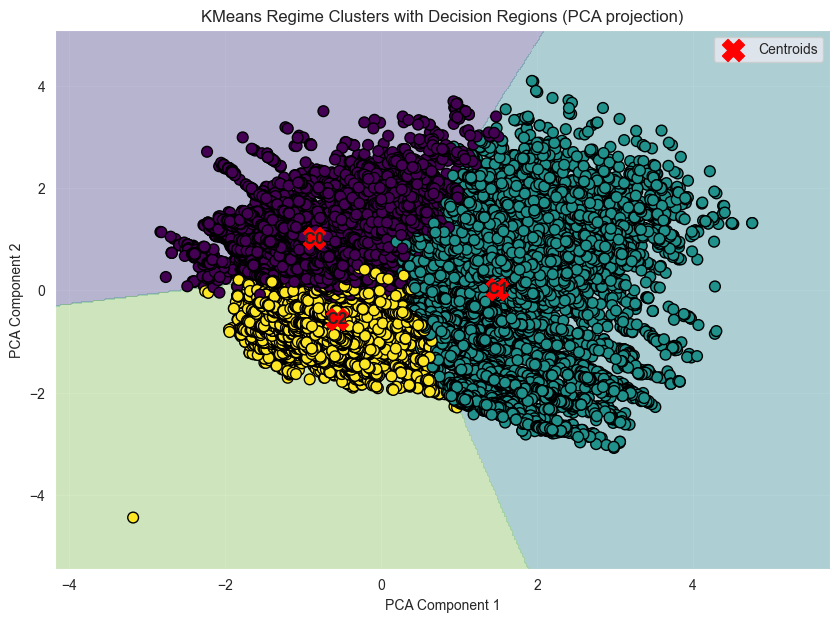
\includegraphics[width=0.9\linewidth]{KMEAN_PCA_simple.png}
    \caption{K Mean Clustering with out any features 2D plot using PCA}
    \label{fig:K Mean with out any features 2D plot using PCA}
\end{figure}

\paragraph{(ii) Feature-Based Representation}

To obtain a more interpretable and compact representation, we construct summary features:

\begin{itemize}
    \item \textbf{Bid-Ask Spread:}
    \begin{equation}
        s_t = P^{ask}_{t,1} - P^{bid}_{t,1}
    \end{equation}

    \item \textbf{Top-of-Book Imbalance:}
    \begin{equation}
        I_t = \frac{v^{bid}_{t,1} - v^{ask}_{t,1}}{v^{bid}_{t,1} + v^{ask}_{t,1} + \epsilon}
    \end{equation}

    \item \textbf{Total Depth:}
    \begin{equation}
        V^{bid}_t = \sum_{i=1}^{L} v^{bid}_{t,i}, \quad
        V^{ask}_t = \sum_{i=1}^{L} v^{ask}_{t,i}
    \end{equation}

    \item \textbf{Depth Slope:}
    \begin{equation}
        S^{bid}_t = \frac{1}{L} \sum_{i=1}^{L} \frac{v^{bid}_{t,i}}{i}, \quad
        S^{ask}_t = \frac{1}{L} \sum_{i=1}^{L} \frac{v^{ask}_{t,i}}{i}
    \end{equation}
\end{itemize}

The resulting feature vector is:
\begin{equation}
    \mathbf{x}_t^{feat} = [s_t, I_t, V^{bid}_t, V^{ask}_t, S^{bid}_t, S^{ask}_t]
\end{equation}

This representation reduces dimensionality while preserving economically meaningful structure.

---
\begin{figure}[ht]
    \centering
    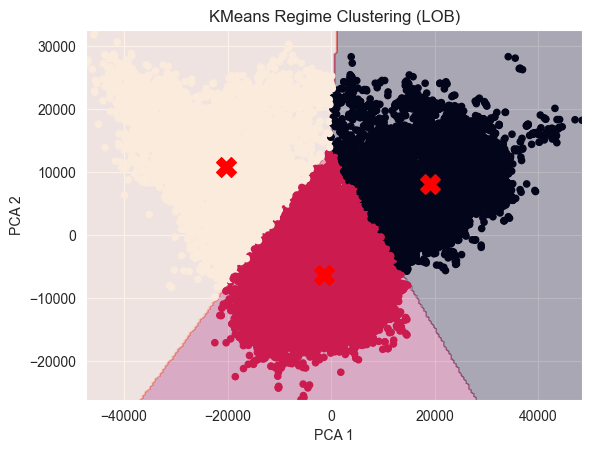
\includegraphics[width=0.9\linewidth]{KMEAN_PCA.png}
    \caption{K Mean Clustering with features- dimension reduced to 2D using PCA}
    \label{fig:K Mean with Features and 2D plot by PCA reduction}
\end{figure}


\subsubsection{Dimensionality Reduction for Visualization}

To visualize high-dimensional LOB states and the resulting clusters, we employ nonlinear dimensionality reduction techniques.

---
\paragraph{PCA (Principal Component Analysis)}

PCA is a linear dimensionality reduction technique that projects high-dimensional data onto a lower-dimensional subspace while preserving maximum variance.

Given centered data $\{\mathbf{x}_i\}_{i=1}^N$ with mean $\bar{\mathbf{x}} = 0$, PCA seeks orthogonal directions (principal components) that maximize the projected variance. The first principal component is obtained as:

\begin{equation}
    \mathbf{w}_1 = \arg\max_{\|\mathbf{w}\| = 1} \sum_{i=1}^{N} (\mathbf{w}^\top \mathbf{x}_i)^2
\end{equation}

This can be equivalently written in terms of the sample covariance matrix:

\begin{equation}
    \Sigma = \frac{1}{N} \sum_{i=1}^{N} \mathbf{x}_i \mathbf{x}_i^\top
\end{equation}

The principal components are given by the eigenvectors of $\Sigma$:

\begin{equation}
    \Sigma \mathbf{w}_k = \lambda_k \mathbf{w}_k
\end{equation}

where $\lambda_k$ are the eigenvalues representing the variance explained by each component.

The projection of the data onto a $d$-dimensional subspace is given by:

\begin{equation}
    \mathbf{y}_i = W_d^\top \mathbf{x}_i
\end{equation}

where $W_d = [\mathbf{w}_1, \dots, \mathbf{w}_d]$ contains the top $d$ eigenvectors.

---

\paragraph{Interpretation:}
PCA identifies directions of maximum variance in the data and provides a linear embedding that preserves global structure. Unlike t-SNE and UMAP, PCA maintains pairwise distances up to linear transformation and allows for exact reconstruction via inverse mapping.

---

\paragraph{Optimization Perspective}

PCA can also be formulated as a reconstruction problem:

\begin{equation}
    \min_{W_d} \sum_{i=1}^{N} \left\| \mathbf{x}_i - W_d W_d^\top \mathbf{x}_i \right\|^2
\end{equation}

subject to $W_d^\top W_d = I$, ensuring orthonormality of the projection directions.

---

\paragraph{t-SNE (t-Distributed Stochastic Neighbor Embedding)}

t-SNE maps high-dimensional data into a low-dimensional space by preserving pairwise similarities. It constructs a probability distribution over pairs of points:

\begin{equation}
    p_{ij} = \frac{\exp(-\|\mathbf{x}_i - \mathbf{x}_j\|^2 / 2\sigma^2)}{\sum_{k \neq l} \exp(-\|\mathbf{x}_k - \mathbf{x}_l\|^2 / 2\sigma^2)}
\end{equation}

and seeks a low-dimensional embedding $\mathbf{y}_i$ such that:

\begin{equation}
    q_{ij} = \frac{(1 + \|\mathbf{y}_i - \mathbf{y}_j\|^2)^{-1}}{\sum_{k \neq l} (1 + \|\mathbf{y}_k - \mathbf{y}_l\|^2)^{-1}}
\end{equation}

The embedding minimizes the Kullback–Leibler divergence:

\begin{equation}
    \min \sum_{i,j} p_{ij} \log \frac{p_{ij}}{q_{ij}}
\end{equation}

\paragraph{Interpretation:}
t-SNE preserves local similarities, making it effective for identifying clusters, but does not preserve global distances.

---
\begin{figure}[ht]
    \centering
    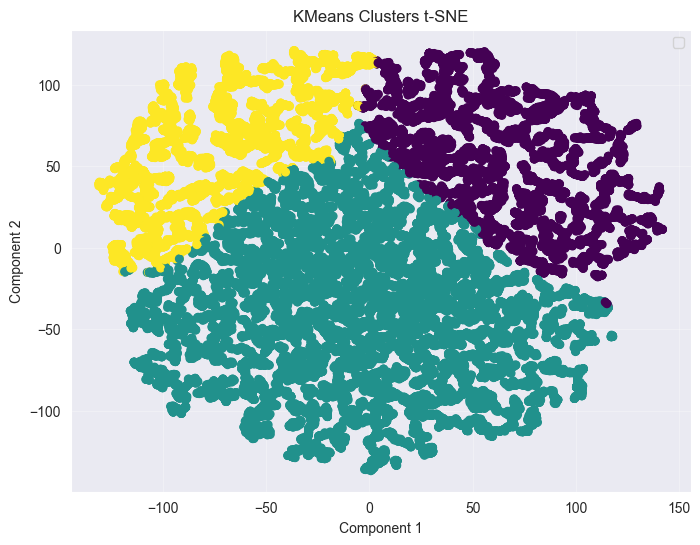
\includegraphics[width=0.9\linewidth]{KMEAN_t-SNE.png}
    % \caption{Bid fill probability}
    \label{fig:K Mean with t-SNE reduction}
\end{figure}
\paragraph{UMAP (Uniform Manifold Approximation and Projection)}

UMAP assumes that the data lies on a low-dimensional manifold and constructs a weighted graph of nearest neighbors. It then optimizes a low-dimensional embedding that preserves this structure.

Formally, UMAP minimizes a cross-entropy between high-dimensional and low-dimensional fuzzy simplicial sets:

\begin{equation}
    \mathcal{L} = \sum_{(i,j)} \Big[ w_{ij} \log \sigma(d_{ij}) + (1 - w_{ij}) \log (1 - \sigma(d_{ij})) \Big]
\end{equation}

where $w_{ij}$ represents edge weights in the high-dimensional graph and $d_{ij}$ is the distance in the embedding.

\paragraph{Interpretation:}
UMAP preserves both local neighborhood structure and partial global geometry, making it suitable for visualizing regime transitions.

---
\begin{figure}[ht]
    \centering
    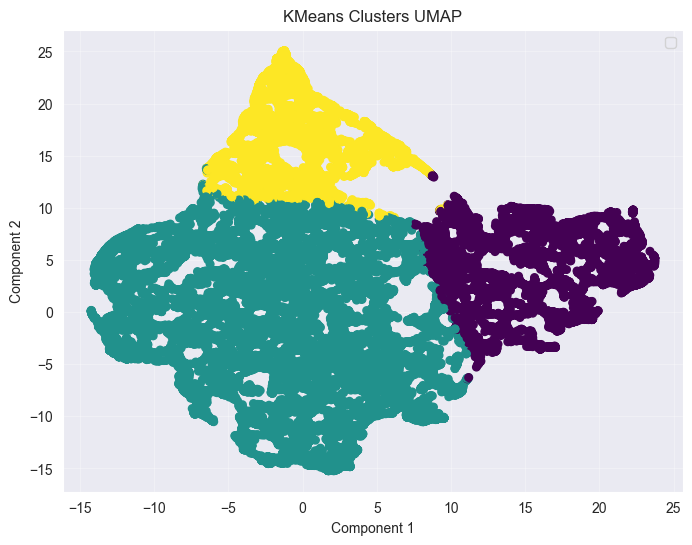
\includegraphics[width=0.9\linewidth]{KMEAN_UMAP.png}
    % \caption{Bid fill probability}
    \label{fig:K Mean with UMAP reduction}
\end{figure}
\subsubsection{Comparison of Methods}

\begin{itemize}
    \item \textbf{KMeans:} Identifies regimes based on Euclidean distance in the original feature space.
    \item \textbf{t-SNE:} Reveals cluster structure by preserving local similarities, but distorts global geometry.
    \item \textbf{UMAP:} Provides a balance between local and global structure preservation, often yielding more meaningful regime separation.
\end{itemize}

---

% \subsubsection{Raw vs Feature-Based Modeling}

% \paragraph{Raw LOB Representation}
% \begin{itemize}
%     \item Pros: Captures full depth information and fine-grained microstructure.
%     \item Cons: High dimensionality, noisy, difficult to interpret.
% \end{itemize}

% \paragraph{Feature-Based Representation}
% \begin{itemize}
%     \item Pros: Interpretable, robust, computationally efficient.
%     \item Cons: May lose subtle structural information present in the full book.
% \end{itemize}

---

\subsubsection{Why Dimension Reductions}

The combination of clustering and dimensionality reduction enables:
\begin{itemize}
    \item Identification of latent market regimes
    \item Visualization of regime separation and transitions
    \item Improved understanding of execution dynamics under different market conditions
\end{itemize}

\paragraph{Comparison with Nonlinear Methods}

\begin{itemize}
    \item PCA preserves \textbf{global variance} but may fail to capture nonlinear structures in LOB data.
    \item Unlike t-SNE, PCA retains \textbf{global geometry}, making distances and directions interpretable.
    \item Compared to UMAP, PCA is computationally efficient but less expressive for complex manifolds.
\end{itemize}

clustering is performed in the original feature space, while UMAP and t-SNE are used solely for visualization and exploratory analysis.


\subsection{Hidden Markov Model for Market Regimes}

To address these limitations, we consider a Hidden Markov Model (HMM), which provides a probabilistic framework for modeling regime dynamics.

\subsubsection{Latent State Process}

Let
\[
S_t \in \{1,2,3\}
\]
denote the latent regime at time $t$. The evolution of regimes is governed by a Markov chain:
\[
P(S_t = j \mid S_{t-1} = i) = P_{ij},
\]
where $P_{ij}$ represents the transition probability from state $i$ to state $j$.

\subsubsection{Observation Model}

Conditional on the latent state, the observed feature vector follows a Gaussian distribution:
\[
Y_t \mid S_t = k \sim \mathcal{N}(\mu_k, \Sigma_k),
\]
where $\mu_k$ and $\Sigma_k$ denote the mean and covariance of state $k$. These parameters are estimated via maximum likelihood methods, typically using the Expectation-Maximization (EM) algorithm.

\subsection{Interpretation of Regimes}

After estimation, the latent states are interpreted as follows:

\begin{itemize}
    \item \textbf{State 0:} Market making regime (stable prices, balanced order flow) ???********
    \item \textbf{State 1:} Upward directional regime (buy-side pressure) ??********
    \item \textbf{State 2:} Downward directional regime (sell-side pressure) ???********
\end{itemize}

\begin{figure}[ht]
    \centering
    
    \begin{subfigure}[b]{0.3\linewidth}
        \centering
        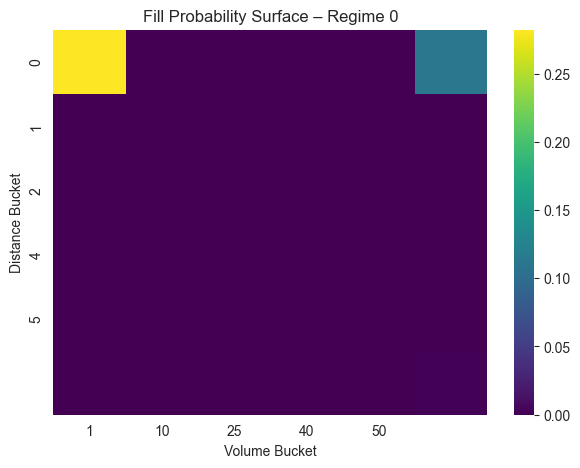
\includegraphics[width=\linewidth]{bid_prob_regimes.png}
        \caption{Regime 0}
    \end{subfigure}
    \hfill
    \begin{subfigure}[b]{0.3\linewidth}
        \centering
        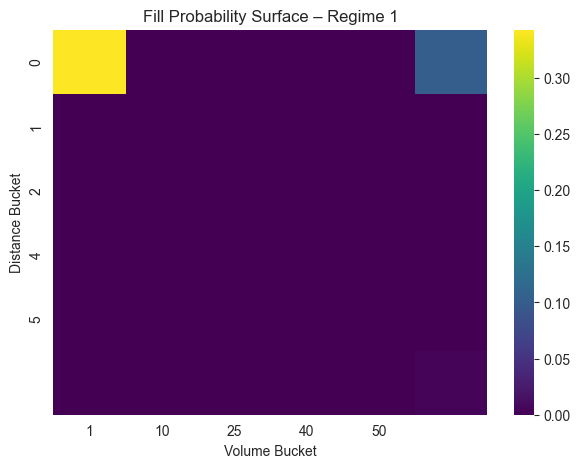
\includegraphics[width=\linewidth]{bid_prob_regime1.png}
        \caption{Regime 1}
    \end{subfigure}
    \hfill
    \begin{subfigure}[b]{0.3\linewidth}
        \centering
        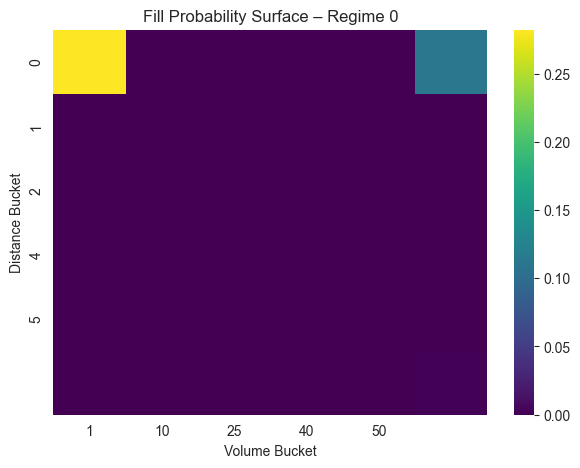
\includegraphics[width=\linewidth]{bid_prob_regimes.png}
        \caption{Regime 2}
    \end{subfigure}

    \caption{Execution probability surfaces of Bids across different market regimes. The first panel corresponds to Regime 0, the second to Regime 1, and the third to Regime 2.}
    
    \label{fig:Bid regime probability surfaces}
\end{figure}

\begin{figure}[ht]
    \centering
    
    \begin{subfigure}[b]{0.3\linewidth}
        \centering
        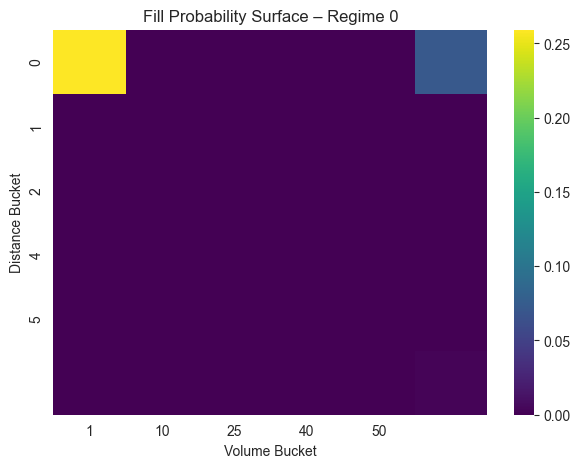
\includegraphics[width=\linewidth]{ask_prob_regimes.png}
        \caption{Regime 0}
    \end{subfigure}
    \hfill
    \begin{subfigure}[b]{0.3\linewidth}
        \centering
        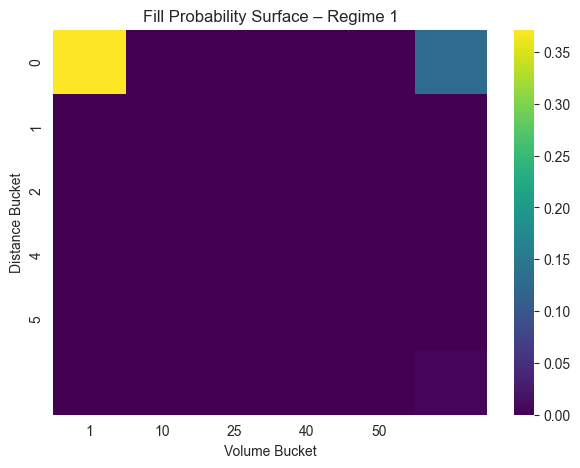
\includegraphics[width=\linewidth]{ask_prob_regime1.png}
        \caption{Regime 1}
    \end{subfigure}
    \hfill
    \begin{subfigure}[b]{0.3\linewidth}
        \centering
        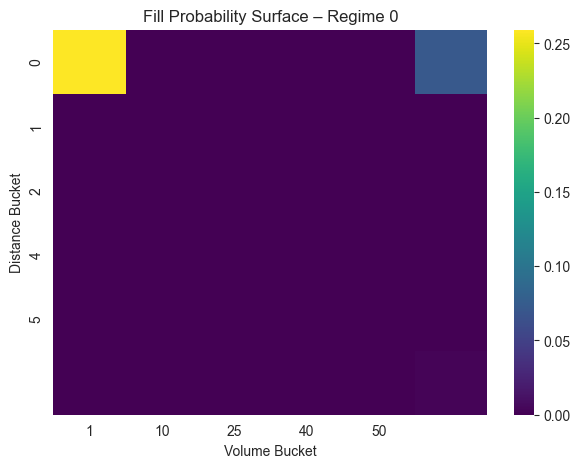
\includegraphics[width=\linewidth]{ask_prob_regimes.png}
        \caption{Regime 2}
    \end{subfigure}

    \caption{Execution probability surfaces of Asks across different market regimes. The first panel corresponds to Regime 0, the second to Regime 1, and the third to Regime 2.}
    
    \label{fig:Ask regime probability surfaces}
\end{figure}

The market making regime corresponds to conditions where price fluctuations remain bounded and liquidity is symmetric, making it favorable for placing passive orders.

\section{Enhanced Feature Engineering}

To further refine regime identification, additional features based on price distance and volume buckets can be incorporated. Let $m_t$ denote the mid-price. The distance of a price level $p$ from the mid-price is defined as:
\[
d(p) = \frac{|p - m_t|}{\text{tick size}}.
\]

We discretize distances and volumes into predefined buckets:

These discretizations allow for a structured representation of liquidity distribution and facilitate modeling of execution probabilities.

\section{Regime-Based Market Making Strategy}

Once regimes are identified, they are incorporated into a market making strategy as follows:

\begin{enumerate}
    \item \textbf{Regime Filtering:} Trading is restricted to the market making regime, avoiding directional regimes that increase adverse selection risk.
    
    \item \textbf{Distance-Based Execution Modeling:} For different price levels (measured as distance from the mid-price), we estimate the probability of order execution within a fixed time horizon.
    
    \item \textbf{Optimal Quote Placement:} Using these probabilities, we determine the optimal bid and ask distances that balance execution likelihood and profit margin.
    
    \item \textbf{Risk Management:} A stopping rule is defined to exit positions, either by booking profits or limiting losses.
\end{enumerate}

This framework ensures that liquidity provision is adaptive to market conditions and grounded in empirical execution dynamics.

\section{Summary}

In this chapter, we developed a framework for regime identification using LOB-derived features. While clustering methods such as $k$-means provide a baseline segmentation, they fail to capture temporal dependencies. The Hidden Markov Model offers a more suitable alternative by explicitly modeling regime transitions and persistence. By combining regime classification with execution probability modeling, we establish a foundation for a robust and adaptive market making strategy.

\chapter{Market Making Price Bands and Execution Modeling}

\section{Overview}

In this chapter, we develop an execution-aware market making framework that integrates regime classification with empirical fill probabilities derived from limit order book (LOB) data. Unlike purely theoretical quoting models, the proposed approach relies on observed execution dynamics to determine optimal quoting distances from the mid-price.

The central idea is to estimate the probability of order execution at different price levels and use this information to construct quoting bands that balance profitability and execution likelihood.

\section{Distance from Mid-Price}

Let $m_t$ denote the mid-price at time $t$, defined as:
\[
m_t = \frac{p_t^{\text{bid},1} + p_t^{\text{ask},1}}{2}.
\]

For any price level $p$, we define its distance from the mid-price in units of ticks as:
\[
d(p) = \frac{|p - m_t|}{\text{tick size}}.
\]

This distance provides a natural way to parameterize quoting decisions, as it directly reflects how far an order is placed from the current market consensus.

\section{Empirical Execution Probability Estimation}

To determine optimal quoting levels, we estimate the probability that an order placed at a given distance from the mid-price will be executed within a fixed time horizon.

\subsection{Counting-Based Estimation}

For each regime $r$, we construct empirical execution probabilities using historical LOB data. The procedure is as follows:

\begin{enumerate}
    \item For each time step $t$ belonging to regime $r$, observe the current LOB snapshot.
    
    \item For each depth level, compute:
    \begin{itemize}
        \item Distance from mid-price $d_t$
        \item Corresponding order volume $v_t$
    \end{itemize}
    
    \item Discretize $(d_t, v_t)$ into predefined distance and volume buckets.
    
    \item Maintain a count of occurrences:
    \[
    N_r(d,v) = \text{number of times a level with distance } d \text{ and volume } v \text{ is observed}.
    \]
    
    \item For each such observation, check whether the order would have been executed within a fixed time horizon $\tau$:
    \begin{itemize}
        \item A bid is considered executed if the future ask price crosses or equals the bid price.
        \item An ask is considered executed if the future bid price crosses or equals the ask price.
    \end{itemize}
    
    \item Maintain execution counts:
    \[
    F_r(d,v) = \text{number of such observations that result in execution}.
    \]
\end{enumerate}

The empirical execution probability is then given by:
\[
P_r(d,v) = \frac{F_r(d,v)}{N_r(d,v)}.
\]

This results in a \textit{probability surface} over distance and volume, conditioned on the regime.

\subsection{Interpretation}

The probability surface $P_r(d,v)$ captures the likelihood that a passive order at a given distance and size will be filled within the specified horizon. Typically:

\begin{itemize}
    \item Orders closer to the mid-price have higher execution probability but lower profit margins.
    \item Orders further from the mid-price have lower execution probability but higher potential profit.
\end{itemize}

This trade-off is central to market making.

\section{Construction of Price Bands}

Using the execution probabilities, we determine feasible quoting regions. In addition, a statistical band based on the stationary distribution of prices can be defined as:
\[
L_t = \mu - k\sigma_{\text{stat}}, \quad U_t = \mu + k\sigma_{\text{stat}},
\]
where $\mu$ and $\sigma_{\text{stat}}$ are the mean and standard deviation of the stationary distribution, and $k$ controls the width of the band.

These bounds represent the region within which prices are expected to fluctuate under stable market conditions.

\section{Conversion to Bid and Ask Quotes}

Since market makers place orders on bid and ask sides, the bands are translated using the prevailing spread:
\[
S_t = A_t - B_t.
\]

The quoting bounds are defined as:
\[
B_t^{\text{bound}} = L_t - \frac{S_t}{2}, \quad
A_t^{\text{bound}} = U_t + \frac{S_t}{2}.
\]

Within these bounds, execution probability surfaces are used to select optimal quoting distances.

\section{Regime-Based Quoting Strategy}

The execution model is applied selectively based on the identified market regime:

\begin{enumerate}
    \item Identify the current regime using the trained regime classification model.
    \item If the regime corresponds to the market making regime, proceed with quoting.
    \item Use the corresponding probability surface $P_r(d,v)$ to determine:
    \begin{itemize}
        \item Optimal bid distance $d_b$
        \item Optimal ask distance $d_a$
    \end{itemize}
    \item Place limit orders at these distances from the mid-price.
\end{enumerate}

In directional regimes, quoting is either avoided or adjusted to account for increased adverse selection risk.

\begin{figure}[ht]
    \centering
    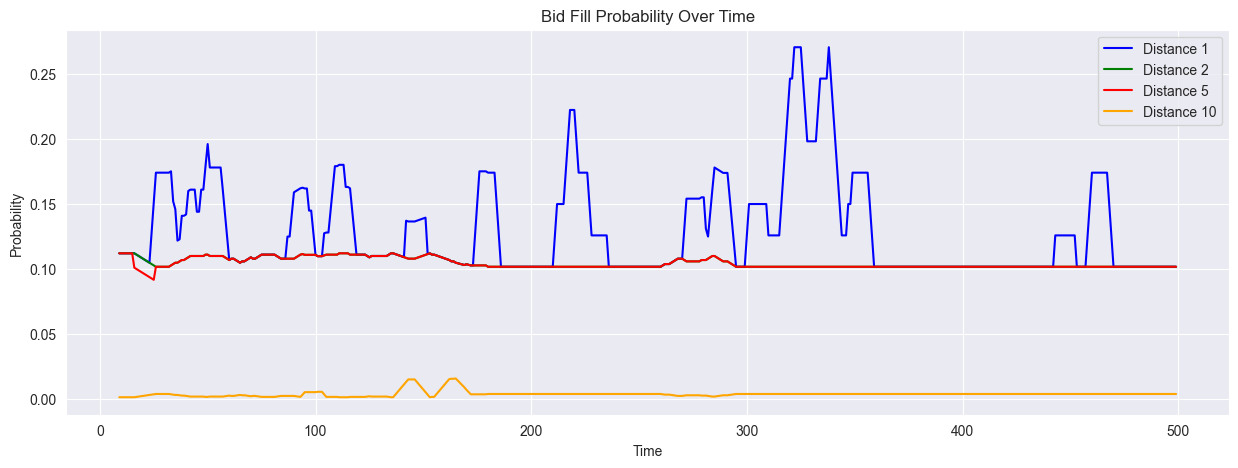
\includegraphics[width=0.9\linewidth]{bid_fill_prob.png}
    \caption{Bid fill probability}
    \label{fig:Probability of fil Bid side}
\end{figure}

\begin{figure}[ht]
    \centering
    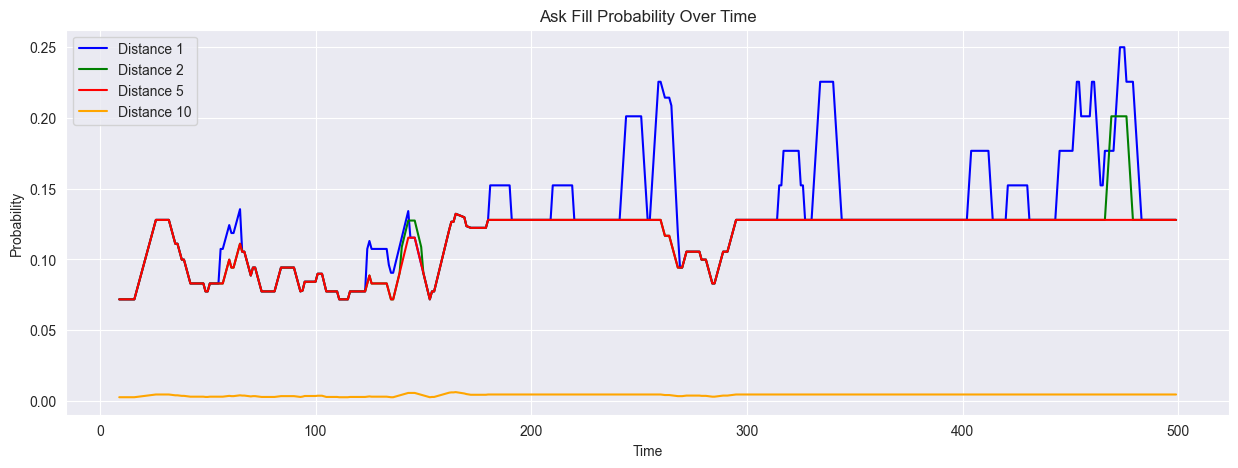
\includegraphics[width=0.9\linewidth]{ask_fill_prob.png}
    \caption{Ask fill probability}
    \label{fig:Probability of fil Ask side}
\end{figure}

\section{Dynamic Recalibration and Online Adaptation}

The execution probabilities described above are initially estimated using a stationary dataset. However, market conditions evolve over time, and static estimates may become outdated.

To address this, the framework allows for dynamic recalibration:

\begin{itemize}
    \item A parallel data pipeline continuously collects fresh LOB data.
    \item Execution probabilities are periodically recomputed using recent observations.
    \item Updated probability surfaces replace older estimates when sufficient new data is available.
\end{itemize}

In practice, the system operates in two modes:

\begin{itemize}
    \item \textbf{Execution Mode:} Uses the most recently calibrated probability surfaces for real-time decision making.
    \item \textbf{Calibration Mode:} Updates model parameters asynchronously using incoming data.
\end{itemize}

This separation ensures that the quoting logic remains stable while still adapting to evolving market conditions.

\section{Comparative Evaluation of Regime Detection Approaches}

The notebook studies regime-dependent execution modeling for a limit order book using a common downstream pipeline: each regime model partitions the snapshot stream, regime-specific bid and ask fill-probability surfaces are estimated over distance and volume buckets, and these surfaces are then queried online to produce level-wise fill probabilities. This common interface makes the comparison meaningful, because differences in output can be attributed primarily to the regime model rather than to changes in the execution-surface construction itself.

\paragraph{Common Experimental Setup.}
Across the notebook, the order book is reconstructed from indexed snapshots with depth $20$, a forecasting horizon of $50$ snapshots, and an exit-time parameter of $25$. The execution surfaces are discretized using distance buckets
\[
\texttt{DIST\_BUCKETS} = [0,1,2,4,5,6]
\]
and volume buckets
\[
\texttt{VOL\_BUCKETS} = [1,10,25,40,50,100].
\]
For each detected regime, separate bid-side and ask-side empirical fill surfaces are estimated as
\[
\hat p_{\text{fill}}(d,v \mid r)
=
\frac{\text{fills in bucket }(d,v)\text{ under regime }r}
{\text{observations in bucket }(d,v)\text{ under regime }r + \varepsilon}.
\]
The comparison therefore focuses on how well each regime model produces coherent, stable, and economically interpretable groupings of book states.

\paragraph{KMeans as the Baseline.}
The original notebook uses $K$Means with three clusters as the baseline regime detector. In the first version, the regime features are microstructure variables such as spread, imbalance, bid depth, and ask depth. In a later version, the feature set is redefined to include mid-price, spread, total bid volume, and total ask volume, with standardization applied before clustering. The notebook also visualizes the resulting regimes in PCA space and overlays decision regions, making $K$Means the most transparent and interpretable model in the current workflow.

The main strength of $K$Means in the notebook is simplicity. The regime assignments are fast to compute, the hard labels map directly into regime-specific surfaces, and the resulting bid and ask probability curves are straightforward to generate. As a baseline, it is effective because it gives an immediate segmentation of the market into a small number of operational states.

However, several limitations are evident from the notebook setup. First, the number of regimes is fixed \emph{a priori} at three, rather than inferred from the data. Second, the clustering is static: every snapshot is assigned independently, with no persistence constraint or transition structure. Third, the inclusion of mid-price in one of the feature definitions risks mixing \emph{price level} with \emph{market regime}, which can make the clusters less about liquidity state and more about where the instrument happened to trade. Finally, the original online probability block uses hard assignments only, so any uncertainty near regime boundaries is discarded.

In short, the notebook shows that $K$Means is useful as a baseline operational segmentation method, but not as a fully satisfactory statistical description of regime structure.

\paragraph{Gaussian Mixture Model (GMM).}
The notebook extends the baseline by training a Gaussian Mixture Model with three components and then querying execution surfaces using \emph{soft regime probabilities}. This is an important improvement over the $K$Means formulation. Instead of assigning each snapshot to a single regime, the GMM estimates posterior probabilities
\[
p(r \mid x_t),
\]
and the execution probability is formed as a weighted mixture of regime-specific surfaces:
\[
\hat p_{\text{fill}}(d,v \mid x_t)
=
\sum_r p(r \mid x_t)\,\hat p_{\text{fill}}(d,v \mid r).
\]

Based on the notebook logic, this is the most statistically coherent approach among the models that are visibly run to completion. It preserves the empirical surface construction while reducing label discontinuity. In practice, this means the fill-probability curves are expected to be smoother over time, because a snapshot near a regime boundary no longer causes a discrete jump from one surface to another. This is particularly appropriate for limit order book states, where liquidity conditions often evolve continuously rather than switching abruptly.

Relative to $K$Means, the GMM offers three clear advantages in the notebook context. First, it allows elliptical clusters rather than spherical ones, which is more consistent with correlated microstructure features. Second, it provides posterior probabilities, which can be used directly in the online fill-probability engine. Third, it avoids some of the brittleness of hard clustering when the feature space is noisy or overlapping.

Its main weakness is that it is still a static cross-sectional model. The GMM improves the geometry of the clusters, but it does not explicitly model regime persistence through time. As a result, if the market transitions slowly but the feature vector oscillates locally, the posterior weights can still fluctuate more than one would like in a temporal execution model.

Overall, the notebook evidence supports the GMM as the strongest \emph{drop-in replacement} for $K$Means. It keeps the same downstream execution-surface architecture while improving statistical flexibility and online smoothness.

\paragraph{Hidden Markov Model (HMM).}
The notebook also trains an HMM with three latent states and builds regime-specific fill surfaces from the inferred state sequence. Conceptually, the HMM is the most natural model for the stated objective of regime detection, because it combines cross-sectional state separation with temporal persistence. In other words, it models not only \emph{what} regime a snapshot belongs to, but also \emph{how} regimes evolve over time.

This matters in a limit order book setting. Many phenomena of interest, such as tight-spread states, stressed liquidity states, and one-sided pressure states, are persistent over short horizons. A static model may repeatedly reassign neighboring snapshots across regimes, whereas an HMM can smooth such behavior through the transition matrix. For execution modeling, that persistence is valuable: if the market is currently in a queue-congested or adverse-selection regime, one expects that state to remain relevant for several subsequent snapshots rather than vanish immediately.

Within the notebook's architecture, the HMM has two important benefits. First, it yields latent states that are more likely to represent genuine market phases rather than merely geometric clusters in feature space. Second, when paired with either hard state prediction or posterior state probabilities, it can support a more stable online execution forecast than $K$Means.

At the same time, the HMM is the most assumption-heavy of the models run in the notebook. Its performance depends on the Gaussian emission structure, the number of latent states, and the adequacy of the selected features for Markovian state representation. If the features do not sufficiently encode order flow, queue dynamics, or volatility state, the temporal smoothing can become an artificial regularizer rather than a true regime mechanism.

Even with that caveat, the HMM is the most compelling choice when the report's notion of ``regime'' is explicitly temporal. Among the notebook approaches, it is the best aligned with the market-microstructure interpretation of a regime.

\paragraph{HDBSCAN.}
HDBSCAN is included in the notebook toolkit but does not appear to have a saved end-to-end output sequence comparable to the $K$Means, GMM, and HMM sections. Nevertheless, its role in the framework is clear. HDBSCAN is attractive because it does not require the number of regimes to be fixed in advance and can naturally identify noise points or irregular density structure.

This is highly relevant for order book data, which often contains sparse, transitory, or anomalous states that do not belong cleanly to a small set of compact clusters. In that sense, HDBSCAN addresses one of the most important structural weaknesses of $K$Means. If the market alternates between a few dense recurring states and many scattered transient states, HDBSCAN can separate the dense regimes and flag the rest as low-confidence or noisy observations.

The main drawback in the notebook context is operational rather than conceptual. HDBSCAN is less convenient for online prediction than $K$Means, GMM, or HMM. New-snapshot assignment may require approximate prediction or nearest-centroid fallback, and noise labels can create gaps in the downstream surface-querying logic. This makes it harder to integrate cleanly into a real-time quoting engine unless a secondary mapping rule is added.

Therefore, HDBSCAN is best viewed as an exploratory regime-discovery tool in the current notebook. It is well suited for discovering whether the three-regime assumption is too restrictive, but it is not yet the cleanest production choice for the execution-probability layer.

\paragraph{Change-Point Detection.}
Change-point detection is also integrated into the regime toolkit, although, like HDBSCAN, it does not appear to have a saved final comparison plot in the current notebook. Its interpretation differs from clustering-based methods. Instead of grouping similar snapshots globally, change-point detection segments the time series into locally homogeneous intervals.

This can be very useful in a trading context, particularly when the market exhibits structural breaks such as a volatility jump, a transition into trend-following order flow, or a sudden widening of spreads. In those cases, the key modeling problem is not necessarily ``which cluster does this snapshot belong to?'', but rather ``has the market entered a new phase?''

For the notebook's fill-surface framework, change-point detection offers a different strength: it can produce execution surfaces conditioned on contiguous market episodes rather than on globally repeated states. This may be advantageous when execution quality depends heavily on recent market context. However, it is weaker as a reusable regime classifier for online inference, since the segment labels are tied to historical breakpoints and not naturally designed for out-of-sample prediction on new snapshots.

Accordingly, change-point detection is most valuable as a diagnostic and structural-analysis tool in the notebook, rather than as the primary online regime engine.

\paragraph{Comparison in Terms of Execution-Surface Usefulness.}
From the notebook's perspective, the downstream objective is not clustering for its own sake, but better fill-probability estimation. Under that criterion, the models can be ranked by how naturally they support regime-conditioned surface lookup.

\begin{itemize}
	\item $K$Means is the simplest and easiest to operationalize, but it is brittle because it relies on hard assignments and fixed geometry.
	\item GMM improves the same pipeline substantially by using posterior regime weights, which makes online fill probabilities smoother and more robust.
	\item HMM is the most economically meaningful when regimes are interpreted as persistent market states; it is likely the best theoretical fit for a sequential execution setting.
	\item HDBSCAN is powerful for discovery and robustness to irregular cluster shapes, but less convenient for online surface querying.
	\item Change-point detection is strongest for identifying structural breaks and episodic shifts, but weakest as a direct reusable classifier for new single-snapshot predictions.
\end{itemize}

\paragraph{Practical Ranking Based on the Notebook.}
Based on the saved notebook workflow and outputs, the practical ranking is as follows:

\begin{enumerate}
	\item \textbf{HMM} for regime modeling when temporal persistence is central to the interpretation of market state.
	\item \textbf{GMM} as the best drop-in statistical upgrade over $K$Means for the existing execution-surface architecture.
	\item \textbf{$K$Means} as a fast, interpretable baseline that is useful for initial segmentation and debugging.
	\item \textbf{HDBSCAN} as an exploratory method for testing whether the regime structure is irregular or contains noise states.
	\item \textbf{Change-point detection} as a complementary structural-break tool rather than the main online regime engine.
\end{enumerate}

\paragraph{Overall Conclusion.}
The notebook demonstrates that regime-conditioned execution surfaces are a promising way to convert market-state information into bid and ask fill probabilities. The baseline $K$Means implementation validates the idea operationally, but its static and hard-clustering nature limits fidelity. The GMM improves the same framework materially by introducing soft regime weighting, while the HMM provides the most conceptually appropriate notion of regime by modeling temporal persistence. HDBSCAN and change-point detection broaden the analysis space further, but in the current notebook they are better interpreted as complementary exploratory tools than as the primary production model.

For a final implementation, the evidence in the notebook suggests that the best path is to retain the empirical surface-based execution layer while replacing the regime engine with either a GMM-based soft assignment model or an HMM-based sequential regime model, depending on whether geometric flexibility or temporal structure is prioritized.

\section{Summary}

This chapter presented a data-driven framework for constructing market making price bands based on empirical execution probabilities. By combining regime classification with distance-based fill probability estimation, the approach enables adaptive and execution-aware quoting. The inclusion of dynamic recalibration further ensures robustness to changing market conditions, making the framework suitable for real-time deployment in electronic markets.



\chapter{Implementation and Future Scope}

\section{Data-Driven Continuous-Time Markov Chain Model for Limit Order Book Dynamics}

\subsection{Overview}

We develop a data-driven continuous-time Markov chain (CTMC) framework to model the dynamics of a limit order book (LOB) using high-frequency market depth data. The model is calibrated directly from empirical snapshots and evolves the queue sizes across discretized price bins.

Let the LOB be observed at discrete times $t = 1, 2, \dots, T$, where each snapshot consists of bid and ask prices and corresponding volumes up to a fixed depth.

---

\subsection{Order Book Representation}

Each snapshot is transformed into a structured representation:

\[
\mathcal{S}_t ={ (p^b_i, q^b_i)_{i=1}^{L},  (p^a_i, q^a_i)_{i=1}^{L} }
\]

where:
\begin{itemize}
\item $p^b_i$, $q^b_i$ denote bid price and volume at level $i$
\item $p^a_i$, $q^a_i$ denote ask price and volume at level $i$
\item $L$ is the depth of the book (e.g., $L=20$)
\end{itemize}

The mid-price is defined as:

\[
m_t = \frac{p^b_1 + p^a_1}{2}
\]

---

\subsection{Mid-Price Smoothing}

To reduce microstructure noise, we define a smoothed mid-price:

\[
\tilde{m}_t = \frac{1}{W} \sum_{k=0}^{W-1} m_{t-k}
\]

where $W=10$ is the rolling window size.

\textbf{Remark:} The smoothed mid-price is used for feature extraction, while raw mid-price is used for bin mapping.

---

\subsection{Price Discretization and Queue Representation}

Prices are discretized into bins relative to the mid-price using a fixed tick size $\delta$:

\[
d^b_i = \left\lfloor \frac{m_t - p^b_i}{\delta} \right\rceil, \quad
d^a_i = \left\lfloor \frac{p^a_i - m_t}{\delta} \right\rceil
\]

We define queue vectors:

\[
Q^b(k) = \sum_{i: d^b_i = k} q^b_i, \quad
Q^a(k) = \sum_{i: d^a_i = k} q^a_i
\]

for bins $k = 0, 1, \dots, N-1$.

---

\subsection{Empirical Arrival Distribution}

The probability of order arrival at bin $k$ is estimated empirically:

\[
p_b(k) = \frac{\sum_{t} \sum_{i} \mathbb{1}(d^b_{t,i} = k)}{\sum_{k} \sum_{t} \sum_{i} \mathbb{1}(d^b_{t,i} = k)}
\]

\[
p_a(k) = \frac{\sum_{t} \sum_{i} \mathbb{1}(d^a_{t,i} = k)}{\sum_{k} \sum_{t} \sum_{i} \mathbb{1}(d^a_{t,i} = k)}
\]

These distributions govern the arrival of limit orders in the CTMC.

---

\subsection{Empirical Time Dynamics}

Instead of assuming exponential inter-arrival times, we use observed time increments:

\[
\Delta t_t = t_{t} - t_{t-1}
\]

This allows the CTMC to evolve using real-time dynamics.

---

\subsection{State Evolution}

At each step, the system evolves as follows:

\begin{enumerate}
\item Sample order side:
\[
\text{side} \sim \text{Bernoulli}(0.5)
\]

---
\item Sample arrival bin:
\[
k \sim p_b(k) \quad \text{or} \quad p_a(k)
\]

\item Update queues using price-time priority:
---

\end{enumerate}

\textbf{Bid arrival:}
\[
Q^a(i^*) \leftarrow Q^a(i^*) - 1 \quad \text{where } i^* = \min { i \leq k : Q^a(i) > 0 }
\]

If no such $i^*$ exists:
\[
Q^b(k) \leftarrow Q^b(k) + 1
\]

\textbf{Ask arrival:}
\[
Q^b(i^*) \leftarrow Q^b(i^*) - 1 \quad \text{where } i^* = \max { i \leq k : Q^b(i) > 0 }
\]

If no such $i^*$ exists:
\[
Q^a(k) \leftarrow Q^a(k) + 1
\]

---

\subsection{Best Bid and Ask}

The best bid and ask bins are defined as:

\[\beta_t = \max { k : Q^b(k) > 0 }, \quad
\alpha_t = \min { k : Q^a(k) > 0 }\]

These define the evolving bid-ask spread.

---

\subsection{Rolling Calibration}

To account for non-stationarity, the model is recalibrated over rolling windows:

\[
\mathcal{S}_{t:t+W} \rightarrow (p_b, p_a, \Delta t)
\]

This allows time-varying arrival dynamics:

\[
p_b(k,t), \quad p_a(k,t)
\]
---

\section{Algorithm Summary}

\begin{enumerate}
\item Convert raw LOB data into structured snapshots
\item Compute mid-price and smoothed mid-price
\item Map prices to discrete bins
\item Initialize queues from the first snapshot
\item Estimate empirical arrival distributions
\item Compute inter-arrival times from data
\item For each time step:
\begin{enumerate}
\item Sample order side and bin
\item Update queues via matching rules
\item Record best bid and ask
\end{enumerate}
\item Periodically recalibrate model using rolling windows
\end{enumerate}

---

\section{Discussion}

This framework provides a fully data-driven approximation to the limit order book dynamics, consistent with the CTMC formulation of Kelly and Yudovina. Unlike classical models, it avoids parametric assumptions on arrival processes and directly leverages empirical order flow, making it suitable for high-frequency trading applications.



\printbibliography
\end{document}
